\documentclass[conference]{IEEEtran}

\usepackage{draftwatermark}
\usepackage[backend=bibtex]{biblatex}

\addbibresource{report.bib}

\begin{document}

	\title{Lag compensation techniques for networked games}
	\author{\IEEEauthorblockN{James Robinson}
	\IEEEauthorblockA{Electronics and Computer Science\\
	University of Southampton\\
	Email: jr4e09@soton.ac.uk}}
	\maketitle

	\begin{abstract}
		In networked multiplayer games, network latency often introduces an unacceptable delay between when the player attempts to take an action and when the action actually takes effect within the game world. In this paper, methods of quantifying the effects of this latency, algorithms that mask its apparent effects, and a selection of novel unified frameworks for lag compensation are explored. Also discussed are the advantages and limitations of each algorithm, along with their potential applications.
	\end{abstract}

	\section{Introduction}

	% Explain what kinds of games we're talking about and general terminology
	% Assume tick-based games

	In gaming, the term ``lag'' refers to the delay between when the user takes an action, and when the action takes effect within the game world. Lag can be introduced by many factors including input device latency, framerate, vsync, and monitor response time, but the most egregious source of lag in networked or online games is the latency between client and server. Although techniques exist to reduce this latency, the fact that data transfer is limited by the speed of light means that this latency can never be completely eliminated.

	Lag reduces player engagement and enjoyment, and furthermore can impact performance in competitive multiplayer games \cite{beigbeder2004effects}. For this reason, most popular online games take measures to reduce the effect of network latency on the player's experience. Such techniques are generally referred to as ``lag compensation'' algorithms. Many such techniques exist, each of which make various tradeoffs that are appropriate for some types of game. Because of the disparate requirements of different genres of game, no ``silver bullet'' solution exists.

	In this paper, I will introduce various state of the art techniques for lag compensation in networked multiplayer games, discussing their advantages and disadvantages, as well as which types of simulation each technique is suited to. I will also present some unified models.

	%\section{Quantifying effects of latency}

	%TODO \cite{beigbeder2004effects} \cite{chen2011perceptual} \cite{claypool2005effect} \cite{fritsch2005effect} \cite{sheldon2003effect} \cite{quax2004objective} \cite{dick2005analysis}

	\section{Dead reckoning}

	The simplest form of client-side lag compensation is ``dead reckoning'' (named for the principle used in navigation). Under this approach, the last known positions and velocities of each game object are used to predict their current position via extrapolation, taking latency into account. For example, given current time $t$, current latency $l$, and a game object with last known position $\hat{s}_{t - l}$ and velocity $\hat{v}_{t - l}$, the predicted position at the current point in time is $\hat{s}_{t} = \hat{s}_{t - l} + l\hat{v}_{t - l}$. Figure~\ref{fig:extrapolation_timeline} shows a timeline of this approach: updates from the server take some amount of time to reach the client, and the client extrapolates game object positions to predict where they are now.

	\begin{figure}
		\centering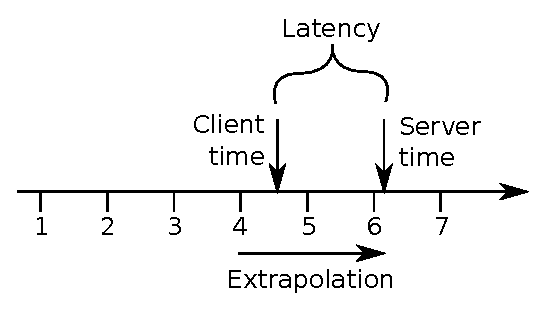
\includegraphics[width=\linewidth]{figures/extrapolation_timeline.eps}
		\caption{A timeline showing extrapolation. The client predicts the current server time based on measured latency, and extrapolates object positions from the position and velocity data in the latest update received from the server ($t = 4$).}
		\label{fig:extrapolation_timeline}
	\end{figure}

	Misprediction errors are very common under this scheme, occurring every time the velocity or bearing of a game object changes. The simplest way to correct misprediction errors is to immediately ``snap'' the object to the correct location once an update arrives from the server, but this can cause very visible visual discontinuities that can be distracting for the player. A less accurate but visually smoother approach is to interpolate between the position that the entity was last rendered at and its current estimated position (as shown in figure~\ref{fig:extrapolation}). This smooths out the visual discontinuities but also further reduces precision.

	\begin{figure}
		\centering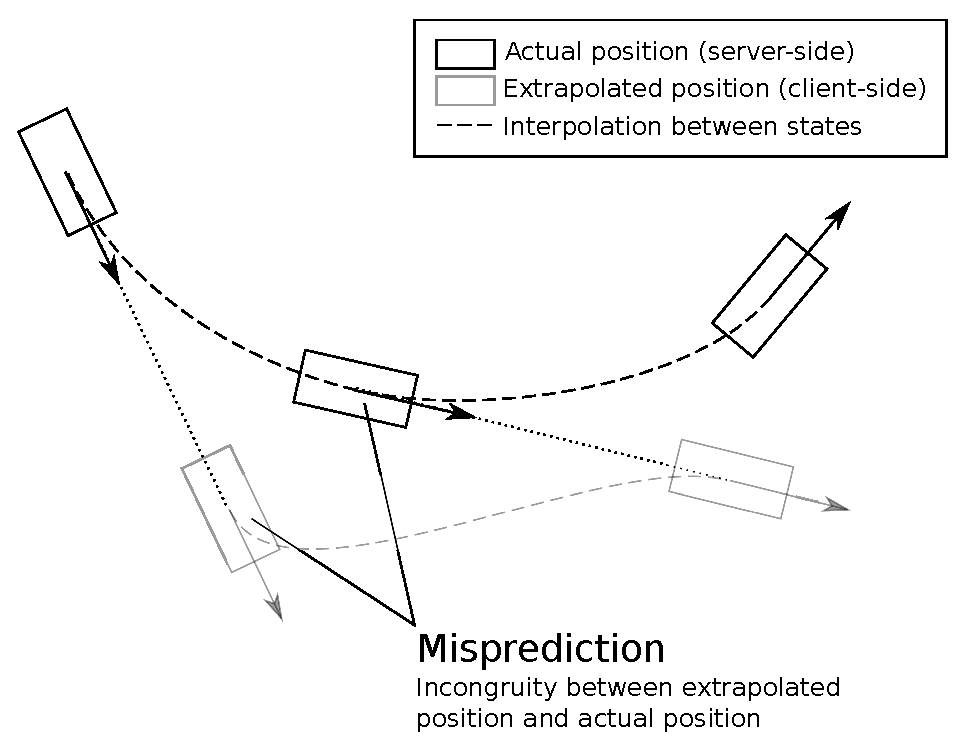
\includegraphics[width=\linewidth]{figures/extrapolation.eps}
		\caption{Misprediction. The client extrapolates object positions based on measured latency in order to predict where they are now. If objects change bearing, misprediction errors occur.}
		\label{fig:extrapolation}
	\end{figure}

	It is important to note that when using this scheme, game objects are very rarely (if ever) rendered at correct, accurate positions. This tradeoff is acceptable for some games, particularly where game objects change velocity or bearing reasonably slowly (for example, cars in a racing game) \cite{pantel2002suitability}, but for games requiring pinpoint accuracy, a better scheme is required.

	% Sometimes use high-order differential coefficients http://www.mine-control.com/zack/timesync/timesync.html

	\Textcite{pantel2002suitability} discusses the suitability of Dead Reckoning schemes for games. The authors classify prediction schemes into two categories: prediction of positions, and prediction of input events. Within these categories they defined 7 different prediction schemes:

	\subsection{Position prediction schemes}

	\begin{enumerate}
		\item Assume objects are moving at a constant velocity, and extrapolate their new positions from their old ones
		\item Assume objects are experiencing constant acceleration, extrapolate their velocity and thus their position
		\item The same as scheme 2, but using a Lagrange polynom of degree 2 (commonly used for interpolation and extrapolation in 3D graphics)
		\item Assume objects are moving at a constant velocity, and use this to plot their trajectory
	\end{enumerate}

	\subsection{Input event prediction schemes}

	\begin{enumerate}
		\setcounter{enumi}{4}
		\item Assume control device (i.e. joystick) positions remain constant, and predict the effect this input will have on the game object
		\item Assume control device velocity remains constant
		\item Assume control device acceleration remains constant, and extrapolate velocity using a degree 2 Lagrange polynom
	\end{enumerate}

	The authors considered applications of these prediction schemes to 3 different types of game: sports games, 3D action games, and simulators/racing games. A simple model was constructed for each type of game in order to assess the viability of each prediction scheme. For sports games, a ``cursor-like steering model'' was used -- game objects steer towards a point within the game world. For both action games and racing games, game objects were assumed to behave like vehicles -- the x axis of the control device manipulates the direction of the game object, and the y axis controls its acceleration. The quality of a prediction scheme was defined as the average deviation between game object positions calculated by the game engine, and their predicted positions.

	The results were surprising: the most complex schemes did not always lead to the best results. For example, scheme 5 was particularly successful despite its simplicity. For sports games, scheme 6 produced the lowest average deviation, with all input-based prediction methods faring reasonably well. For action games, scheme 7 fared best. Because of the proprietary physics engine used in the racing game example, it was only possible to evaluate position-based prediction. Schemes 2 and 3 performed equally well.

	There are a number of issues with the approach presented in the paper:

	\begin{itemize}
		\item The model used to simulate action games is fundamentally unrealistic; characters in a first-person shooter do not behave like vehicles. Instead, players are able to move freely in any direction, rather than being constrained to motion in the direction they're facing. Players in shooter games also tend to move far more eratically than in the demonstration from the paper.
		\item Using input prediction schemes for a competitive multiplayer action game might be infeasible for the same reason that input prediction failed for racing/simulation games in the paper: most action games use proprietary physics engines, many of them involving incredibly complex interactions between game objects and the environment (explosions, destructible terrain, etc.). Prediction is very difficult in such games, hence the ubiquity of the delayed presentation approach described in section~\ref{sec:delayed_presentation}.
	\end{itemize}

	The results presented in the paper are misleading at best -- prediction likely does not work as well for action games as the authors claim. However, the novel prediction techniques presented for both racing games and sports games do perform better than the naive approach, and might see use in future titles.

	\Textcite{Simpson2000} describes a technique for improving the accuracy of dead reckoning via the use of a novel clock synchronisation algorithm. The author evaluates the possibility of using existing algorithms such as NTP, but concludes that because NTP is so difficult to implement and takes so long to converge, it is unsuitable for a game in which the player expects to be able to ``jump in'' rather than waiting for clock synchronisation to converge.

	The proposed clock synchronisation algorithm is essentially a moving average latency calculation built upon TCP. The client periodically sends ``time request'' packets timestamped with the local time to the server, and the server sends back a timestamped response. The client subtracts the time when the response was received from the time when the request was sent in order to determine the round-trip time between client and server, halving this to obtain the latency, and takes the delta between the timestamp of the sent message and the timestamp of the received message, adding the latency to produce a clock delta. This process is repeated a number of times to produce an ordered list of clock deltas, and the median is taken. Samples that are further than 1 standard deviation from the mean are discarded. Finally, the local clock is adjusted based on this delta in order to synchronise the local and remote clocks.

	This algorithm is intended to be used in tandem with timestamped updates to improve the accuracy of dead reckoning algorithms in networks with high variance in packet delivery times (``jitter''). It was implemented in \emph{NetStorm, Islands At War} (a commerial real-time strategy game) with good results, typically obtaining synchronisations less than 100ms.

	\Textcite{aggarwal2004accuracy} furthered this idea and developed an improvement for the dead reckoning algorithm, focusing on extrapolation accuracy, testing their new approach in the game \emph{BZFlag}.

	This new approach is primarily applicable to distributed games, in which there is no authoritative server, or in which players are authoritative over the positions of their own characters. The algorithm involves clients generating dead reckoning vectors (position and velocity data) for game objects under their control at every update, broadcasting these vectors to every other client. Without clock synchronisation, and without knowledge of the latency between any given pair of peers, it is impossible to estimate when a given update packet was sent. For this reason, a clock synchronisation algorithm is used to ensure the clocks on each client are consistent, and the dead reckoning vectors are augmented with timestamps so that the recipient can accurately plot the object's path.

	The authors implemented their new technique in BZFlag, and added instrumentation to trace the paths that game objects take both on the sender and receiver, so that the accuracy of the simulation could be measured. It was found that there were significant quantitative improvements under the new approach, even with latency as high as 100ms. Unfortunately this technique is not necessarily directly applicable to all action games; BZFlag players control tanks that are constrained to traditional vehicle movement (much like a racing game), whereas action games in which the player is on foot tend to have far more eratic movement patterns.

	\Textcite{cai1999auto} describe an auto-adaptive dead reckoning algorithm for distributed interactive simulations, which might also be applicable to peer to peer games. In general, distributed simulations built using dead-reckoning must make a tradeoff between prediction accuracy and bandwidth; by sending fewer position updates bandwidth may be conserved, at the cost of prediction accuracy. Many distributed systems operate by withholding position updates until the error between the actual position of an entity and its predicted position goes over some fixed threshold. The benefit of this approach is that by altering the threshold, the tradeoff between accuracy and bandwidth can be adjusted. However, not all clients need accurate location data for all entities (for example, a player does not need particularly accurate position information for another player a significant distance away), and so using a fixed threshold for every game object is inefficient.

	The authors address this limitation by introducing the concept of \emph{threshold levels}. Each game object has a defined \emph{area of interest} (AoI), sometimes called the \emph{reachability region}, which is a circle around the game object whose radius is usually related to the type of object. The area of interest represents the region in which dead reckoning accuracy is important from the perspective of that game object. Furthermore, each game object has a \emph{sensitive region} (SR); if another game object moves within a game object's SR, a collision is likely to occur. The authors define 4 different threshold levels based upon the interactions between the AoI and SR of the game objects and the relative distance between them.

	This algorithm requires each simulator to maintain the last known positions of all game objects, both local and remote. After each update of the game object controlled by a simulator, the true position of the entity is compared with the predicted positions at other simulators - if the difference is greater than the threshold, then a position update is sent.

	The primary drawback of this approach is memory consumption: in a system with $N$ entities controlled by $N$ simulators, each simulator must maintain not only its own state, but also the last known position of the controlled game object by each of the other $N - 1$ simulators.

	\section{Local lag}

	\Textcite{mauve2004local}

	\begin{itemize}
		\item Voluntarily decrease responsiveness in order to eliminate short-term inconsistencies
		\item Makes inconsistencies less likely but can't completely eliminate them
		\item Time-warp algorithm to repair inconsistencies as they appear
		\item Developed a simple demonstration program used to verify theoretical observations
		\item Discrete = changes in state in response to user-initiated operations
		\item Continuous = changes in state may occur due to passage of time without requiring exhange of information
		\item Rigorous definitions of consistency and correctness out of scope of this report
		\item Instead of immediately processing events, they are delayed for a certain amount of time before being executed (often configurable by the player as an option labeled "frame delay")
		\item Work conducted in the area of system response time suggests a highest acceptable response time of 80-100ms \cite{teal1992performance} \cite{shneiderman1984response} \cite{card1983psychology}, so local lag should generally be below this value (citations 11-13 in paper)
		\item For specific applications it might make sense to measure this
		\item Packets might still arrive late if the network latency is higher than the local lag, or due to packet loss or variable delivery times (jitter)
		\item Time warp algorithm repairs the state, too long to reproduce here
		\item In the time warp synchronization scheme [10], snapshots of the game state are taken before the execution of each event. When there are late events, the game state is rolled back to one of the previous snapshots, and the game is reexecuted with the new events.
		\item Keep a record of previous states, and pick the state that immediately precedes the earliest pending operation
		\item Known problems: visual artefacts caused by the correction applied by timewarp algorithm. These can take many forms: objects jumping from one place to another, characters temporarily appearing to be alive when they're actually dead. No general solution to this, must be solved on a case-by-case basis
		\item Implemented a very simple game to demonstrate this algorithm, tested with simulated network delay
		\item Commonly used in fighting games, popular implementation is GGPO
	\end{itemize}

	\section{Delayed presentation}
	\label{sec:delayed_presentation}

	An interesting approach to lag compensation is used in first-person shooter games built upon the Source game engine (including the Counter-Strike series and the Team Fortress series, among others), as described by \textcite{bernier2001latency}. The engine was built using a traditional client-server model in which the server is authoritative over game state. Clients are relatively simple: they sample user input and package it into timestamped packets which get sent to the server. The server handles simulation logic (including movement, physics and hit registration), and broadcasts the new location data of each game object after each update to each client.

	Instead of using dead reckoning to predict object positions based on their last known locations, clients in the Source engine instead buffer received updates and render the world as it appeared some time in the past. By doing this, the client ensures it always has at least 2 real, historic updates to interpolate between, thus completely eliminating misprediction errors (but at the cost of further increasing latency). Packet loss is implicitly handled by the algorithm -- the client attempts to keep 3 updates buffered at all times, and so in the case of single packet loss it still has two valid states to interpolate between. A timeline illustrating this approach is given in figure~\ref{fig:interpolation_timeline}. If the client runs out of buffered packets (due to packet loss or server error), it falls back to extrapolation/dead reckoning.

	In order to mimimise apparent latency, the client predicts the movement of the player's character while awaiting confirmation of each movement from the server. It is important to minimise discrepancies between client and server in the prediction logic, and so identical movement code is shared between the client and the server.

	Due to the communication latency between client and server, the server's update messages are stale by the time they reach the client, and the client's update messages are stale by the time they reach the server. The artificial delay introduced on the client-side to allow interpolation to work futher increases this latency. If this delay were not accounted for, players would have to ``lead'' their targets by an amount proportional to their latency and the interpolation delay, which is an unacceptable compromise. In the Source engine, therefore, the server keeps a record of the past second of game states. When an update packet arrives from a client, the server uses this historical data to ``rewinds time'' an amount based on the player's latency and the interpolation period in order to see what the player saw when the command was sent, and the command is then executed in this context.

	This approach can cause temporal paradoxes from the perspectives of some players. For instance, if a player with high latency shoots a player with lower latency just as the lower latency player hides behind cover, the shot will still register and the player who hid behind cover will die. From the perspective of the defending player, it appears as if they have been ``shot around a wall'', but from the perspective of the attacking player, they scored a fair hit. In practice these issues are rarely noticable due to the very short time periods involved, and so the tradeoff is considered acceptable for most purposes.

	The delayed presentation approach has been used in many commercially successful games with excellent results.

	\begin{figure}
		\centering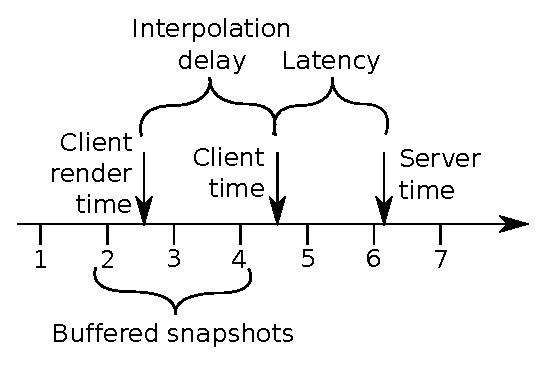
\includegraphics[width=\linewidth]{figures/interpolation_timeline.eps}
		\caption{A timeline showing delayed presentation. The client buffers updates received from the server for a short period instead of displaying them immediately. Under this scheme the client always has at least two snapshots to interpolate between, eliminating the need for prediction/dead reckoning.}
		\label{fig:interpolation_timeline}
	\end{figure}

	\section{Latency equalisation}

	\cite{yu2012latency}

	\begin{itemize}
		\item Has applications to teleconferencing and online trading as well as gaming
		\item In addition to requiring low end-to-end latency, such applications also benefit from minimising the difference between the latencies of multiple clients.
		\item Existing QoS services allow end-to-end latency to be controlled, but this is insufficient if we need bounded delay difference across multiple clients
		\item Proposed Latency EQualization (LEQ) service, equalises perceived latency for all participating clients
		\item Uses some routers along the network as hubs to redirect packets along paths with similar end-to-end delay
		\item Only a small number of hubs are required
		\item Significantly reduces delay difference in synthetic tests
		\item Compromise between end-to-end delay and delay difference between clients (fast clients have to slow down), maybe not appropriate for all applications
		\item Incrementally deployable in today's networks, requiring only software modification to existing routers
		\item Has not yet seen widespread adoption
	\end{itemize}

	\section{Timelines: A unified framework}

	\Textcite{savery2013timelines} describe a unified approach to lag compensation built upon the concept of \emph{timelines}. Timelines are a data structure that ``expose the temporal dimension of shared data'', allowing the programmer to specify the known value of a variable at a specific point in time, and automatically and transparently handling the interpolation or extrapolation required to predict the value of that variable at a point in time where its actual value is unknown. Timelines are fully replicated, and each client has its own timeline object for each portion of the simulation it is interested in. This allows the programmer to manipulate the flow of time, or to create divergent timelines for different players.

	The timelines model simplifies and unifies existing lag compensation algorithms, allowing dead reckoning, smooth correction of misprediction errors, delayed input, and time-offsetting to be implemented with relative ease. The model addresses 3 primary issues that lag compensation techniques must handle.

	Firstly, the \emph{stale message problem} -- that there is no way to know when a received message was sent, due to variance in network delivery times (``jitter''). The timelines framework solves this problem by clock synchronisation and the inclusion of timestamps in each message.

	Secondly, the \emph{stale state problem} -- games typically display updates to the user very frequently (60 times per second for most titles), but in order to conserve bandwidth network updates are often sent at a lower frequency. In some games updates might also be delayed if a client can detect that another client can extrapolate the position of an entity accurately via dead reckoning. The client must therefore have some method of compensating for missing or suppressed updates (interpolation), and the ability to keep track of remote state.

	Thirdly, the \emph{frame of reference problem} -- some games deliberately alter the player's frame of reference (for example Half-Life 2, which uses delayed presentation). This increases the predictability of entities, but also allows state to diverge between players (i.e. each player has their own unique view of the world). To provide consistency and prevent cheating, the server must be able to ``rewind time'', to recreate a remote client's state when that remote client took an action. This is trivial within the timelines framework.

	Finally, the \emph{multiple times at once problem} -- some lag compensation techniques (for example, smooth correction of misprediction errors), require that the client be able to know past, present and future values of a given variable at the same time. By exposing the temporal dimension of the data to the programmer, such algorithms become trivial to implement.

	The model has some known limitations:

	\begin{itemize}
		\item It does not support multiple clients updating (writing) the same timeline at the same time, since each client might overwrite the values the other wrote. This could potentially be fixed by adding synchronisation primitives to the framework, but it is unclear when such a problem would arise in a real-world game, since typically only one is authoritative over a particular game object.
		\item It's unsuitable for serialization of large objects, since the entire shared object must be sent over the network with every update. By using custom serialisation functions that only transmit the fields of the object that have changed (``delta encoding'') it is possible to sidestep this problem, but further work is required to generalise this to apply to every type of object.
		\item Command type data (e.g. ``jump'', ``shoot'') is not handled in the timelines model since there is no meaningful way to ``interpolate'' or ``extrapolate'' such data. Instead, the application is expected to maintain a separate queue for such messages, or to use an event-driven approach.
	\end{itemize}

	An additional potential limitation of the model that is not addressed in the paper is that it does not assume a tick-based game engine. In the timelines framework, a doubly linked list is used to store known state values tagged by time. Finding the value of a shared variable at a particular point in time therefore requires traversal of the list, which involves a pointer dereference for each step (a highly cache-unfriendly operation). In most networked multiplayer games, the server operates on a fixed tick-rate, and values may only be updated during a tick. In such games, it might make more sense to represent timelines as arrays, where the array index represents the tick, and the value at that index represents the value of the variable at that tick. This could potentially reduce the time complexity of get and set operations against the timeline for tick-based games.

	\section{Conclusions}

	\begin{itemize}
		\item No catchall solution
		\item Lots of dead reckoning algorithms, but added complexity does not always equate to significantly increased accuracy
		\item Delayed presentation is still the standard for first-person shooters. Works well even at comparatively high latency but causes temporal paradoxes
		\item Dead reckoning works well if game objects accelerate/decelerate slowly (racing games), but not if movement is erratic
		\item Local lag is popular for fighting games. Works well on low latency connections but since it doesn't actually eliminate lag it's bad for high latency networks
		\item All of these have drawbacks that would be unacceptable for certain applications
		\item Could see the move towards unified frameworks like Timelines that abstract away the differences between these techniques, potentially allowing them to be combined where necessary
		\item Improved network speed would help, but data cannot travel faster than light so there will always necessarily be lag
	\end{itemize}

	\printbibliography

\end{document}
